% Generated by build_isp_paper.py; compile with XeLaTeX-compatible Tectonic or XeLaTeX.
\documentclass[UTF8,a4paper,zihao=-4,fontset=none]{ctexart}
\usepackage[a4paper,top=2.4cm,bottom=2.3cm,left=2.4cm,right=2.4cm]{geometry}
\usepackage{fontspec}
\usepackage{xeCJK}
\usepackage{amsmath,amssymb}
\usepackage{graphicx}
\usepackage{booktabs}
\usepackage{array}
\usepackage{float}
\usepackage{enumitem}
\usepackage{caption}
\IfFontExistsTF{Times New Roman}{\setmainfont{Times New Roman}}{\setmainfont{TeX Gyre Termes}}
\IfFontExistsTF{SimSun}{\setCJKmainfont{SimSun}}{\setCJKmainfont{FandolSong}}
\setlength{\parindent}{2em}
\linespread{1.18}
\captionsetup{font=small,labelfont=bf}
\begin{document}
\pagestyle{plain}
\begin{center}
{\LARGE\bfseries 基于 ACE-Step 的音乐风格生成系统：LoRA 续训与参考音频条件建模}\\[0.5em]
{\large ACE-Step Music Style Generation via LoRA Continuation and Reference-Audio Conditioning}\\[0.8em]
EDM-Adapter 项目组
\end{center}
\begin{abstract}
音乐生成是智能语音处理从语音识别、语音合成扩展到通用音频理解与生成的重要任务，但通用文本到音乐模型仍难以稳定复现特定 EDM 制作风格。本文提出一个基于 ACE-Step 的双路径系统：一方面采用参数高效 LoRA 续训，在冻结 MusicDCAE、UMT5 与大部分扩散 Transformer 的前提下，将可训练范围由最后 2 个 block 扩展到最后 4 个 block；另一方面设计无训练参考音频条件链路，对上传音频进行标准化、声学特征提取和参考 latent 编码，实现音色与频谱质感迁移。实验使用 231 个原始音频源构建 6016 条 8 秒样本，训练/验证/测试划分为 4833/557/626；LoRA 从 step=120 续训 840 步至 step=960，可训练参数约 2.02M，仅占 3.9B 基础模型的约 0.05\%。同 seed 自动评估表明系统能够在固定随机起点下生成 baseline 与 LoRA 对照音频，并记录 RMS、低频比例、BPM、起音密度和 latent 去噪轨迹。结果说明，该系统在 4 卡 RTX 4090 工作站上实现了真实参数适配、无训练参考音频条件生成和可复现实验记录。
\end{abstract}
\noindent\textbf{关键词：}智能语音处理；文本生成音乐；ACE-Step；LoRA 续训；参考音频条件；潜变量扩散

\noindent\textbf{Abstract:} Music generation extends intelligent speech processing from recognition and synthesis to general audio representation and generation. This paper presents an ACE-Step system with two separated paths: LoRA continuation fine-tuning and training-free reference-audio conditioning. The prototype builds 6016 eight-second clips, continues the adapter from step 120 to step 960, and trains about 2.02M parameters while freezing the 3.9B foundation model. Automatic same-seed evaluation records waveform outputs, acoustic metrics, denoising traces, and visualization artifacts for reproducible analysis.

\section{引言}
智能语音处理的研究对象正在从传统语音波形扩展到更广义的音频信号，包括音乐、环境声、多说话人场景以及跨模态音频生成。在这些任务中，系统不仅要理解语义，还要处理采样率、响度、频谱、节奏、瞬态、长时结构和波形重建等信号问题。扩散模型在图像与音频生成中已经证明了强大的概率建模能力[1-4]，而 MusicGen、MusicLM 与 ACE-Step 等模型进一步推动了文本到音乐生成的发展[5-7]。

\subsection{智能语音处理中的音乐生成任务}
从课程主题看，音乐生成并不是脱离语音处理的孤立任务。语音识别、语音合成、说话人转换和音乐生成都需要把连续波形映射到某种中间表征，再在该表征上进行条件建模、重建与评价。区别在于，语音识别更关注音素、词和语义序列，语音合成更关注文本到自然语音的韵律和声学参数，而音乐生成同时关心节奏周期、和声张力、音色层次、混音空间和长时段落推进。因此，本文将音乐风格生成作为智能语音处理的扩展任务，重点讨论波形标准化、声学潜变量、频谱统计、起音检测和生成过程可视化如何共同作用于一个可运行系统。

在实际应用中，用户提出的“生成某种风格”往往不是一个单一文本标签。以 EDM 为例，风格既包括鼓组音色、低频侧链、合成器明亮度、混响空间和母带响度，也包括编曲层面的 build-up、drop、breakdown 和 loop 边界。这些因素同时分布在时域、频域和潜变量空间中，单纯依靠 prompt 难以稳定控制。因此，必须引入能够处理原始音频信号的前端、能够适配模型内部表示的微调方法，以及能够记录生成轨迹的实验框架。

\subsection{基础模型微调的背景与必要性}
然而，现有基础模型在具体音乐风格上仍存在三个限制。第一，单纯 prompt 很难稳定约束 EDM 中的四拍底鼓、sidechain bass、明亮钢琴和 drop 能量推进。第二，即使在本地多卡工作站上，直接全量更新数十亿参数模型仍会带来显著显存、存储和实验管理成本，因此需要 LoRA 等参数高效微调方法[8]。第三，用户上传参考音频时，希望迁移音色和混音质感而不是复制旋律；如果只从参考音频提取提示词，就无法体现真实的智能音频处理过程。

基础模型微调的核心动机是缩小通用训练分布与目标数据分布之间的差距。ACE-Step 这类模型在大规模音乐数据上预训练，已经具备文本到音乐的通用能力，但它的默认分布不一定偏向某个小数据域中的制作习惯。若只改变提示词，模型仍会沿着预训练分布中概率较高的路径采样，导致输出在鼓组、低频、合成器层次和段落结构上漂移。微调则直接改变去噪网络在目标条件下的局部决策，使模型在同样的 seed、prompt 和采样器下产生不同的声学轨迹。

全量微调虽然表达能力强，但对于 3.9B 参数级别的音乐扩散模型并不经济：不仅训练显存和优化器状态开销较大，保存多个实验版本也会快速消耗存储空间。LoRA 的优势在于把权重更新约束为低秩增量，只训练少量矩阵参数，从而保留基础模型的通用音乐知识，同时在目标风格方向上施加可控偏移。因此，本文不把微调视为简单“继续训练”，而是把它作为智能音频生成系统中连接目标数据集、声学 latent 和扩散去噪决策的关键适配机制。

\subsection{研究问题与技术路线}
本文目标是在本地 4 卡 RTX 4090 工作站环境中实现一个可运行、可复现、可解释的 ACE-Step 音乐风格生成系统。系统同时保留长期风格适配路径和临时参考音频路径，并在网页端用任务队列、元数据、波形图、频谱图和 latent 去噪轨迹记录完整生成过程。本文重点验证：参数高效适配是否可以稳定改变基础音乐模型的目标风格偏好，是否可以将上传音频转换为声学条件，是否可以用可视化证据解释生成过程。

围绕上述目标，本文把系统拆分为三个可检验问题。第一，LoRA 续训是否能够在不破坏基础模型泛化能力的情况下改变目标风格倾向；第二，参考音频能否以声学特征和潜变量形式参与生成，而不是被退化为文字标签；第三，网页端记录的任务队列、参数、latent 轨迹和音频诊断图能否支撑重复实验与错误定位。这样的拆分使微调路径和无训练路径在工程上互不冲突，在论文实验中也能分别评价。

本文主要贡献如下：1）提出并实现 ACE-Step LoRA 续训方案，将早期 2-block adapter 扩展为 4-block 末端去噪适配，最终得到 step=960 的 LoRA bundle；2）实现无训练参考音频条件生成链路，将参考音频以标准化波形、客观声学特征和 MusicDCAE latent 的形式注入推理流程；3）构建网页任务队列与科研式可视化，使同 seed 对照、采样步数、latent 轨迹和音频诊断可以逐项复现。全文组织如下：第 2 节评述相关工作，第 3 节给出问题定义与系统框架，第 4 节介绍方法，第 5 节报告实验，第 6 节讨论局限，第 7 节总结全文。

\begin{figure}[H]
\centering
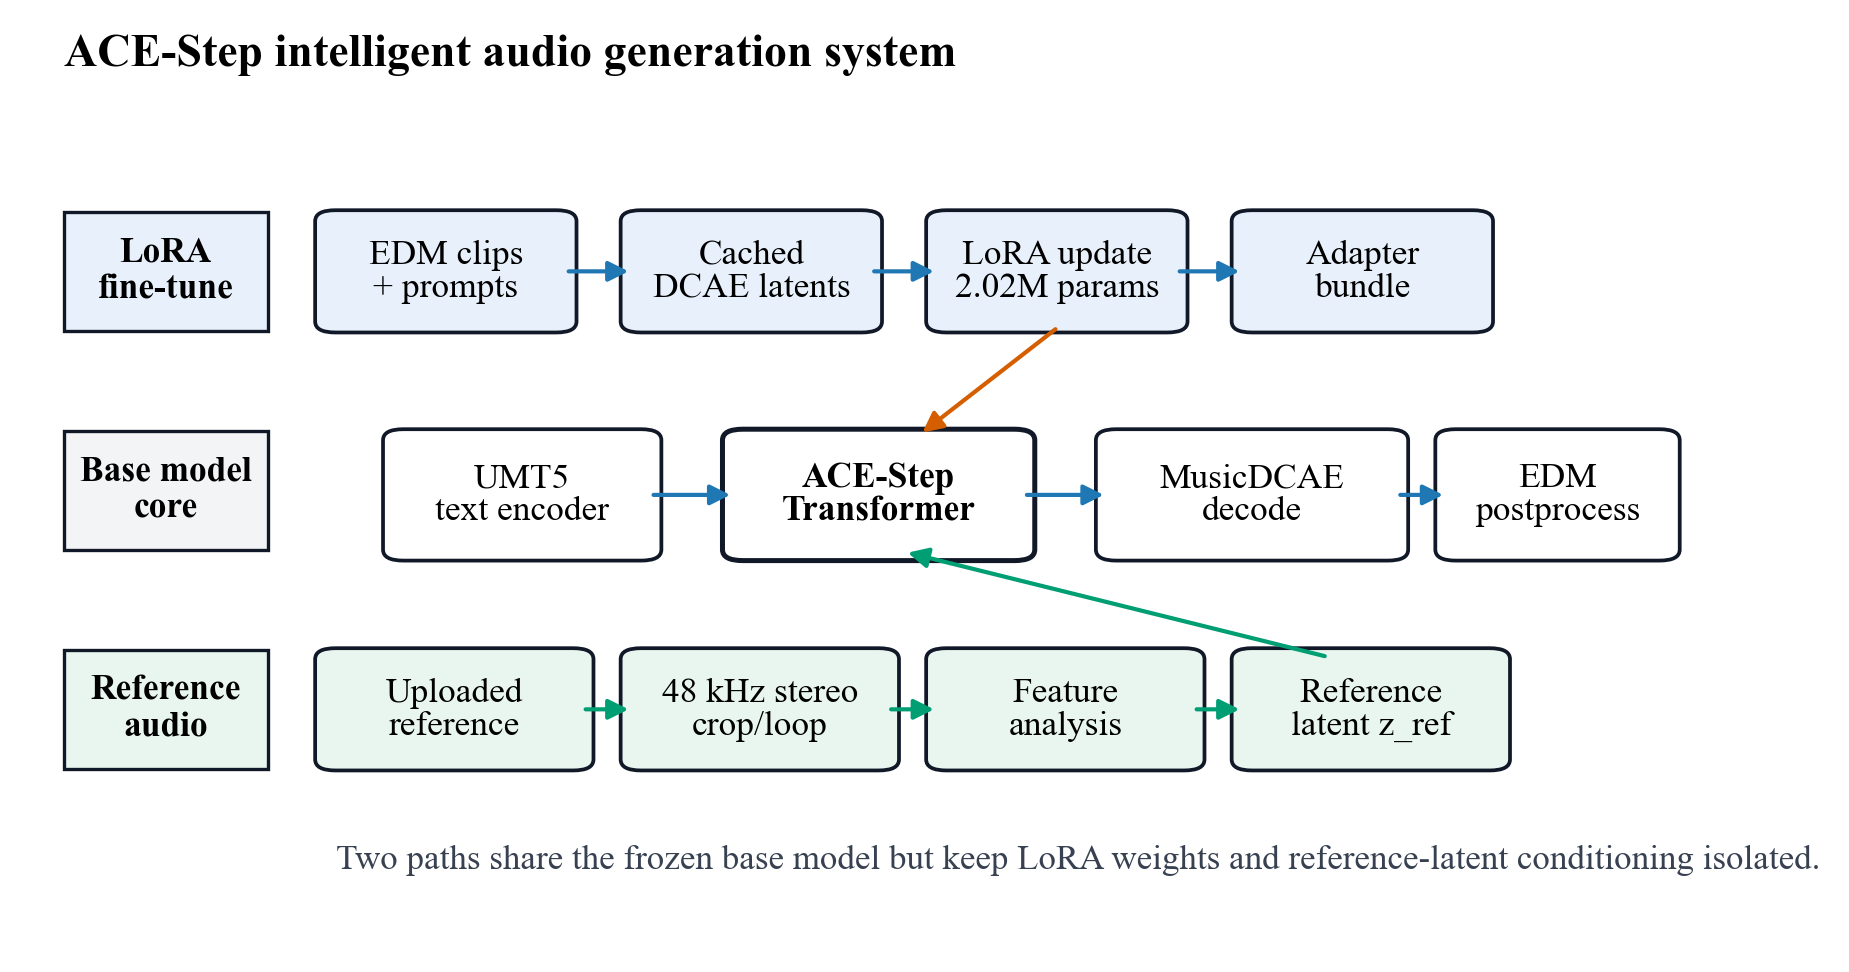
\includegraphics[width=0.92\linewidth]{assets/fig1_system_architecture.png}
\caption{系统总体架构。系统包含 LoRA 续训与无训练参考音频两条路径，二者共享 ACE-Step 基础模型但权重加载和参考 latent 条件相互隔离。}
\end{figure}
\section{相关工作}
\subsection{潜变量扩散与音频生成}
DDPM 将生成过程建模为逐步加噪和反向去噪过程[1]，Latent Diffusion 进一步把扩散过程转移到压缩潜空间，从而降低高维信号生成成本[2]。AudioLDM 与 AudioLDM 2 将类似思想用于文本到音频生成，说明在声学潜空间中进行扩散建模可以兼顾质量与效率[3,4]。本文沿用潜变量扩散思想，但研究重点不是重新训练完整扩散模型，而是在已有 ACE-Step 基础模型上进行风格适配。

\subsection{文本生成音乐基础模型}
MusicGen 使用离散音频表示和自回归建模实现可控音乐生成[5]，MusicLM 展示了文本描述到长时音乐片段的生成潜力[6]。ACE-Step 则将 DCAE 压缩、自回归外的扩散生成、线性 Transformer 与音乐语义表征结合，面向较长音乐生成、歌词对齐和多任务音乐编辑[7]。这些模型共同证明了文本到音乐生成的可行性，但在个人数据域、特定制作风格和本地工作站部署中仍需要额外适配机制。

\subsection{参数高效微调与音频表征}
LoRA 通过冻结预训练权重并学习低秩矩阵增量，使大模型适配不再需要更新全部参数[8]。对于音乐模型，音频压缩和表征质量同样关键；神经音频压缩模型能够保留高保真波形信息[9]，CLAP、MERT 等音频-文本或音乐表征模型则提升了跨模态语义对齐能力[10,11]。本文使用 ACE-Step 内部 MusicDCAE latent 作为训练与参考条件载体，并使用 librosa 提取 BPM、起音密度和频谱特征[12]。

参数高效微调方法的价值不仅在于节省显存，还在于降低实验变量数量。对于音乐风格生成，如果同时更新声学编码器、文本编码器和扩散主干，输出差异可能来自表征漂移、语义条件漂移或去噪网络漂移，难以定位。LoRA 将可训练部分限制在少量线性投影旁，使实验更接近“在固定基础能力上学习风格偏移”。这种设计适合课程实验中的可解释性要求，也适合在网页端以轻量 adapter 形式管理多个版本。

\subsection{参考音频条件与风格迁移}
参考音频条件生成与传统音乐风格迁移相关，但目标并不完全相同。传统风格迁移常希望在保留内容结构的同时改变音色或表现形式，而本文的无训练路径要求“音色和制作质感相似，但旋律与和弦不要直接复制”。这意味着参考信号不能以高强度重构方式进入模型，否则输出会接近原曲；也不能只转写为提示词，否则参考音频中真实的频谱、响度和瞬态结构会丢失。

因此，本文把参考音频拆成两类条件：一类是可解释的低维声学统计量，例如 BPM、低频比例、RMS、谱质心和 onset 密度；另一类是 MusicDCAE 产生的高维参考 latent，用于携带更细粒度的音色和混音质感。低维特征负责约束宏观属性，高维 latent 负责提供声学纹理，但通过 ref\_strength 控制其影响范围。这种设计体现了智能语音处理中的“信号分析 + 表征学习 + 条件生成”三段式流程。

\subsection{音频生成评价}
音乐生成评价通常需要结合主观听感和客观指标。Fréchet Audio Distance 与 PANNs 等方法提供了音频分布层面的评价思路[13,14]，但在小规模课程实验中，完整感知评价成本较高。因此本文采用可复现实验记录作为基础评价：固定 seed 的 baseline/LoRA 对照、RMS、低频比例、BPM、起音密度、波形/频谱可视化和 latent 轨迹。

需要强调的是，客观指标不能直接等价于“好听”或“像某种风格”。RMS 只能反映平均能量，低频比例只能粗略刻画 bass 和 kick 的能量分布，BPM 估计会受到鼓点清晰度和瞬态检测的影响，onset 密度也可能把噪声瞬态误判为起音。本文使用这些指标的目的不是替代人工听感，而是建立可复现的诊断基线：当输出被认为浑浊、没有旋律或音质变差时，可以回查频谱、波形和 latent 轨迹，判断问题更可能来自采样步数、参考强度、LoRA 权重、后处理还是随机初态。

\section{问题定义与系统设计}
给定文本提示 c\_text、可选歌词 c\_lyric、随机种子 s，以及可选参考音频 x\_ref，系统目标是生成一段音乐波形 y。LoRA 路径通过训练参数 θ\_L 改变基础模型在目标 EDM 数据域中的生成偏好；参考音频路径不更新任何参数，而是把 x\_ref 转换为参考 latent 与声学特征。两条路径在网页端以不同 task kind、不同缓存键和不同输出目录保存，避免实验变量混淆。

\subsection{双路径解耦设计}
系统设计的第一条原则是将长期参数适配与临时参考条件解耦。LoRA 微调改变的是模型参数，适用于目标数据集稳定、风格需要长期复用的场景；无训练参考音频改变的是推理输入，适用于用户临时上传一首参考曲并希望借鉴其音色或混音质感的场景。如果把两条路径混合在一个默认推理链路中，生成结果的差异可能来自 LoRA、参考 latent、prompt 或 seed，实验结论会变得不可解释。

因此，网页端在任务级别保存 mode、adapter、reference\_audio、ref\_strength、seed、infer\_step、guidance\_scale 和 scheduler 等关键变量。同 seed 对照任务只改变 LoRA 开关，不引入参考音频；参考音频任务默认不加载 LoRA，只评估参考条件对基础模型的影响。这种隔离策略使每个实验问题只对应一个主要变量，符合科研论文中控制变量实验的基本要求。

\subsection{系统数据流与状态记录}
系统从输入到输出共有四类数据流。第一类是训练数据流，从原始音频切片到 latent 缓存、文本 token 和控制曲线；第二类是微调权重流，从 checkpoint 到 LoRA bundle、manifest 和网页模型下拉项；第三类是推理任务流，从用户参数到生成音频和后处理结果；第四类是诊断数据流，包括日志、波形图、频谱图、latent 轨迹和 JSON 指标。这些数据流共同保证论文中的实验结果可以追溯到具体文件，而不是只依赖主观描述。

\begin{table}[H]
\centering
\caption{双路径生成任务的状态隔离}
\small
\begin{tabular}{p{0.22\linewidth}p{0.32\linewidth}p{0.36\linewidth}}
\toprule
任务类型 & 允许改变的变量 & 固定或隔离的变量 \\
\midrule
LoRA 同 seed 对比 & adapter on/off & seed、prompt、duration、infer\_step、scheduler、后处理链 \\
LoRA 权重强度分析 & lora\_weight & adapter 版本、seed、文本条件、采样步数 \\
参考音频新旋律 & reference latent、ref\_strength & LoRA 权重关闭，旋律复制强度受限 \\
参考重构模式 & ref\_strength>=0.85 & 标记为重构实验，不与新旋律生成混淆 \\
网页可视化 & 任务状态实时更新 & 每个任务独立目录，日志和指标不可覆盖 \\
\bottomrule
\end{tabular}
\end{table}
\begin{table}[H]
\centering
\caption{系统模块与智能语音处理任务对应关系}
\small
\begin{tabular}{p{0.22\linewidth}p{0.32\linewidth}p{0.36\linewidth}}
\toprule
模块 & 处理对象 & 作用 \\
\midrule
音频标准化 & 训练切片/上传音频 & 统一采样率、声道、时长和响度，降低输入分布差异 \\
声学特征分析 & 波形 & 提取 BPM、RMS、低频比例、谱质心和 onset 密度 \\
MusicDCAE 编码 & 波形到 latent & 将高维音频压缩为扩散模型可处理的潜变量 \\
LoRA 续训 & ACE-Step Transformer & 仅更新低秩 adapter，学习目标风格偏移 \\
参考 latent 条件 & 上传音频 latent & 在不训练的情况下约束音色、频谱和局部质感 \\
可视化评价 & latent/波形/频谱 & 记录去噪轨迹和音频诊断，支持复现实验 \\
\bottomrule
\end{tabular}
\end{table}
\section{方法}
\subsection{数据构建与声学前端}
原始数据包含 231 个音频源，其中 203 个源文件通过清洗，最终形成 6016 条 8 秒训练片段。每个片段被统一为 ACE-Step 兼容的采样率和声道格式，同时生成文本条件、段落标签、能量标签、BPM、控制曲线、MusicDCAE latent 和文本 token。数据划分采用 song-level split，避免同一首歌的相邻片段同时进入训练集和测试集。

\begin{equation}
x'(t)=\mathrm{Norm}(\mathrm{Resample}(x(t))),\quad z=E_{\mathrm{DCAE}}(x')
\end{equation}
式(1)表示声学前端处理：原始波形先经过重采样和幅度归一化，再由 DCAE 编码为潜变量 z。该步骤对应智能语音处理中常见的前端标准化与特征表征思想，只是本文的目标从语音识别扩展为音乐风格生成。

\begin{table}[H]
\centering
\caption{数据集构建与缓存资产}
\small
\begin{tabular}{p{0.22\linewidth}p{0.32\linewidth}p{0.36\linewidth}}
\toprule
项目 & 数值/设置 & 说明 \\
\midrule
训练片段 & 6016 条，每条 8 s & 固定长度样本便于 latent 缓存和批处理训练 \\
数据划分 & train/val/test=4833/557/626 & 使用 song-level split 降低数据泄漏 \\
latent 缓存 & 6016 份，failures=0 & 减少训练阶段重复编码成本 \\
文本 token & 6016 份 & 保证文本条件与声学 latent 一一对应 \\
控制曲线 & T x 36 维 & 包含节拍相位、低频、onset、loop 边界等声学控制量 \\
\bottomrule
\end{tabular}
\end{table}
训练片段长度选择 8 秒是质量与效率之间的折中。过短的片段容易只包含局部鼓点或过门，难以学习完整的和声与段落推进；过长的片段会增加 latent 长度、显存占用和批处理等待时间。8 秒片段通常能够覆盖一个或两个 EDM 小节组，既包含稳定节奏，又能在本地多卡环境下进行批量续训。对于生成端，网页仍允许设置 15 秒或更长时长，训练片段长度不直接限制最终输出长度。

文本条件并非只写入固定触发词。每个训练样本还包含 BPM、能量段落、loop 边界、乐器或制作元素等描述，使模型在去噪时同时看到语义条件和声学 latent。这种做法的目的不是让模型记住某一首歌，而是让 adapter 学会“哪些声学结构通常与哪些文本条件共同出现”。为了降低数据泄漏，划分时按原始音频源分组，而不是按切片随机打乱。

\begin{table}[H]
\centering
\caption{声学前端特征及其用途}
\small
\begin{tabular}{p{0.22\linewidth}p{0.32\linewidth}p{0.36\linewidth}}
\toprule
特征 & 计算对象 & 系统用途 \\
\midrule
BPM & onset envelope & 约束节奏速度并检查 prompt 是否被执行 \\
RMS & 标准化波形 & 判断响度是否稳定，辅助发现削波或能量塌缩 \\
低频比例 & <250 Hz 频带 & 刻画 kick/bass 能量占比，定位低频浑浊 \\
谱质心 & 短时频谱 & 估计明亮度和高频纹理变化 \\
onset 密度 & 瞬态检测 & 反映鼓点和节奏事件密度 \\
latent 统计 & MusicDCAE latent & 记录去噪过程是否逐步收敛 \\
\bottomrule
\end{tabular}
\end{table}
\subsection{LoRA 续训架构}
早期配置只训练最后 2 个 Transformer block，约 1.12M 参数，能够产生可听差异但风格与音质仍不稳定。本次架构将可训练作用域扩展为最后 4 个 Transformer block，同时保留 conditioning 模块与 final layer 的 LoRA。目标模块包括 Q/K/V 与输出投影、cross-attention 投影、genre/speaker embedder、t\_block.1、final\_layer.linear。基础模型、MusicDCAE 与 UMT5 始终冻结。

\begin{figure}[H]
\centering
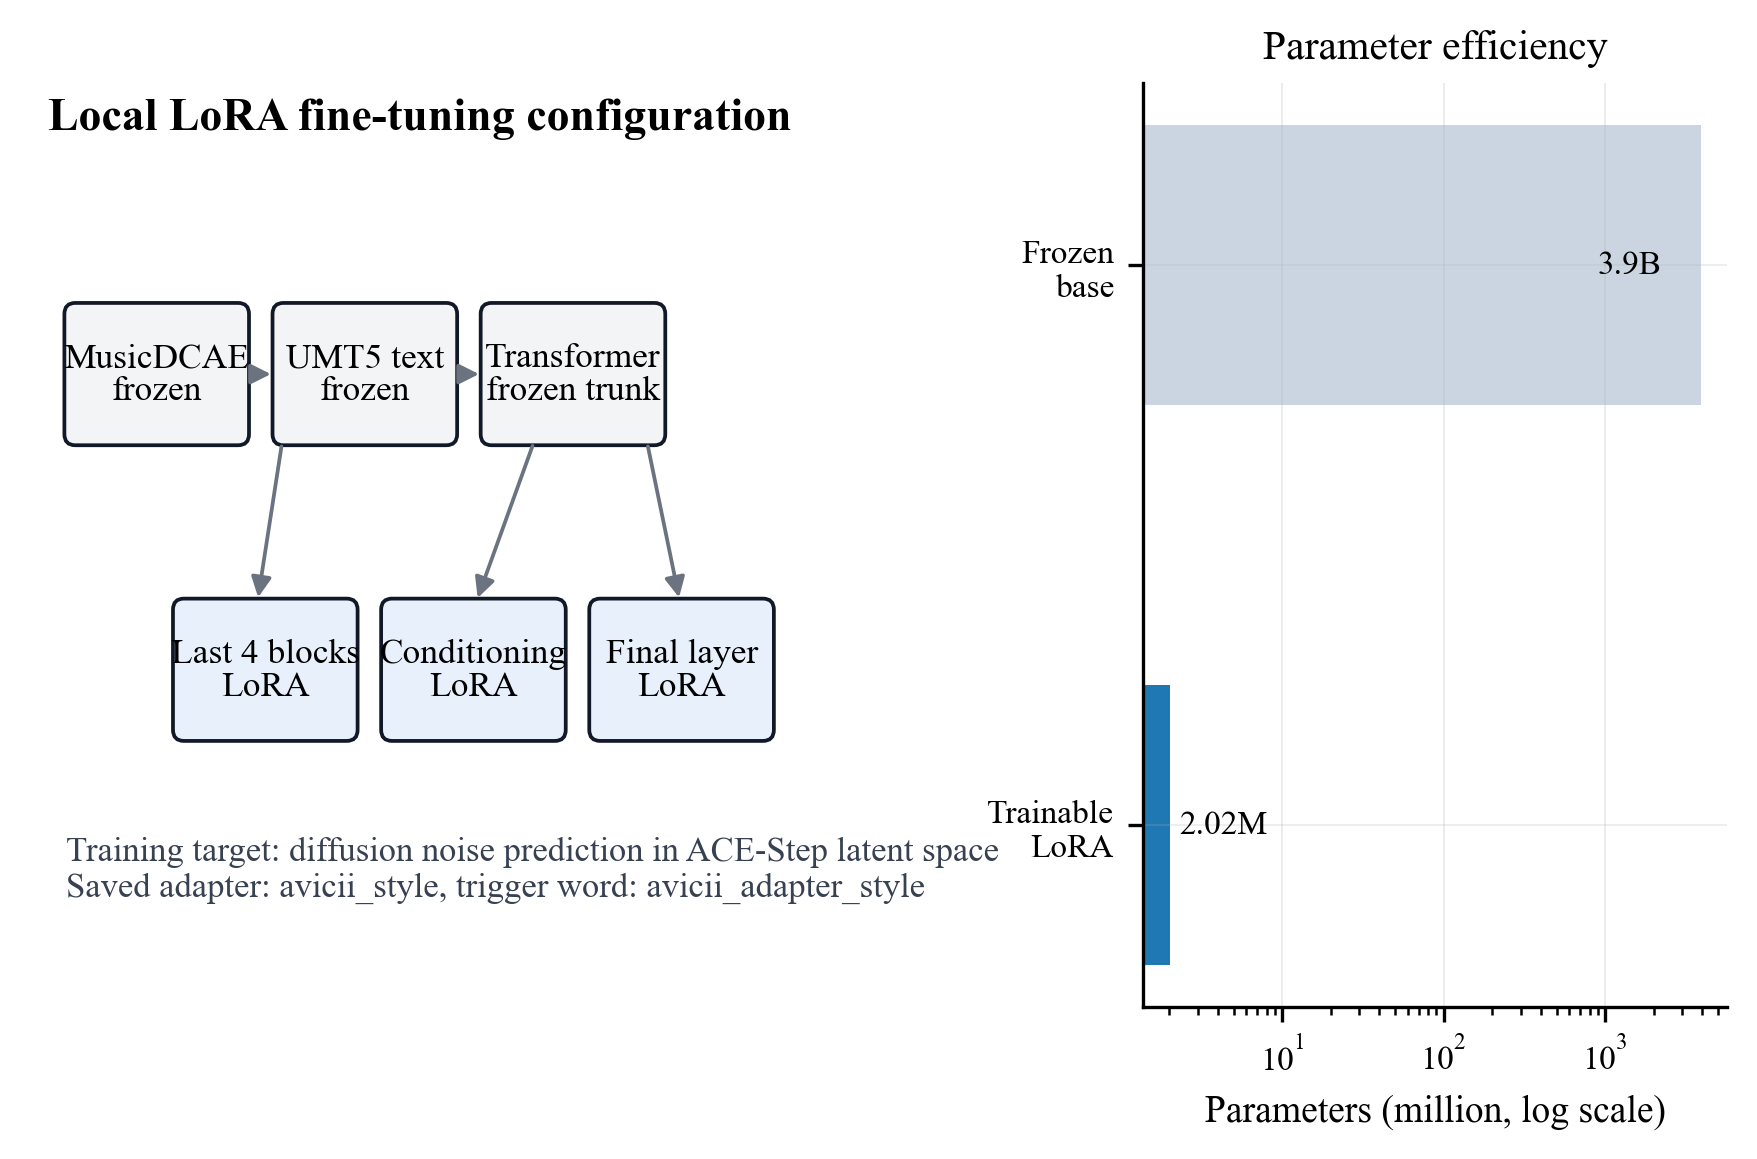
\includegraphics[width=0.92\linewidth]{assets/fig2_lora_finetuning.png}
\caption{本地 LoRA 续训结构。训练只更新末端低秩 adapter，基础声学编码器、文本编码器和 Transformer 主体保持冻结。}
\end{figure}
\begin{equation}
W=W_0+\Delta W,\quad \Delta W=\frac{\alpha}{r}BA
\end{equation}
\begin{equation}
\mathcal{L}(\theta_L)=\mathbb{E}\left[\left\|\epsilon-\epsilon_{\theta}(z_t,t,c_{text};\theta_L)\right\|_2^2\right]
\end{equation}
式(2)为 LoRA 权重增量形式，其中 r=8、alpha=16；式(3)为潜变量扩散训练损失。本次训练从 step=120 adapter 初始化，继续优化 840 个 local step，最终保存 step=960。学习率由早期 5e-4 降为 2e-4，warmup 提升到 40，gradient clipping 设置为 0.35，以减轻小批量训练中的不稳定。

\begin{table}[H]
\centering
\caption{新旧 LoRA 架构与训练配置对比}
\small
\begin{tabular}{p{0.22\linewidth}p{0.32\linewidth}p{0.36\linewidth}}
\toprule
项目 & 早期配置 & 本次配置 \\
\midrule
初始化 & 随机 LoRA & 加载 step=120 后续训 \\
训练范围 & 最后 2 block + 条件层 & 最后 4 block + 条件层 \\
参数量 & 约 1.12M & 约 2.02M \\
训练数据 & 短步数试训 & 完整 train=4833 clips \\
优化器设置 & lr=5e-4, warmup=10 & lr=2e-4, warmup=40 \\
正则化 & dropout=0.03 & dropout=0.01, prompt dropout=0.02 \\
产物 & step=120 & step=960 \\
\bottomrule
\end{tabular}
\end{table}
\begin{table}[H]
\centering
\caption{LoRA 续训流程}
\small
\begin{tabular}{p{0.22\linewidth}p{0.32\linewidth}p{0.36\linewidth}}
\toprule
阶段 & 输入 & 输出 \\
\midrule
初始化 & ACE-Step base 与 step=120 LoRA & 载入 avicii\_style adapter \\
冻结 & MusicDCAE、UMT5、Transformer 主体 & 仅保留 LoRA 参数可训练 \\
采样 & 训练集 latent、文本 token、噪声时间步 & 构造 z\_t 与条件 c\_text \\
优化 & 式(3)损失、AdamW、梯度裁剪 & 更新 θ\_L \\
保存 & 每 100 step checkpoint & LoRA bundle 与 manifest \\
\bottomrule
\end{tabular}
\end{table}
从训练稳定性角度看，本次架构调整并不是简单把训练步数增加。早期 2-block 配置只在最末端少量张量上施加增量，容易出现风格偏移不充分和局部补偿过强的问题；扩展到最后 4 个 block 后，adapter 可以影响更长的去噪决策链，使节奏、音色和频谱结构的调整不完全堆叠在最后输出层。与此同时，学习率降低和 warmup 增加可以减少继续训练初期对已学 adapter 的破坏。

LoRA dropout 从 0.03 降到 0.01 的原因也与小数据风格适配有关。过高 dropout 会抑制 adapter 对细粒度音色和混音质感的学习，导致生成结果虽然不容易过拟合，但听感上缺少明确风格方向；过低 dropout 则可能让模型记住触发词或局部片段。本文同时加入 style prompt dropout=0.02，使训练过程中少量样本不完全依赖触发词，从而鼓励模型从声学 latent 和上下文条件中学习风格线索。

\begin{table}[H]
\centering
\caption{LoRA 训练稳定性策略}
\small
\begin{tabular}{p{0.22\linewidth}p{0.32\linewidth}p{0.36\linewidth}}
\toprule
策略 & 解决的问题 & 实现方式 \\
\midrule
续训初始化 & 随机 adapter 需要重新学习早期风格方向 & 从 step=120 bundle 加载 θ\_L \\
扩大末端 block & 只改最后层导致补偿局部化 & last\_n\_blocks 从 2 扩展到 4 \\
降低学习率 & 继续训练初期可能破坏已学偏移 & lr=2e-4, warmup=40 \\
梯度裁剪 & 小 batch 下梯度峰值造成音质不稳 & gradient\_clip=0.35 \\
轻量 dropout & 欠拟合或只记触发词 & LoRA dropout=0.01, prompt dropout=0.02 \\
\bottomrule
\end{tabular}
\end{table}
\subsection{无训练参考音频条件生成}
参考音频路径不训练、不加载 LoRA，也不把上传音频简化为提示词。系统将参考音频复制到任务目录，执行 48 kHz 双声道标准化、裁剪或循环补齐、BPM/RMS/低频比例/谱质心/onset 特征提取，并编码参考 latent。在“风格音色（新旋律）”模式中，系统默认 ref\_strength=0.32，并限制在 0.18 到 0.45，以降低旋律复制概率；歌词为空时强制使用 [instrumental]。

针对直接使用完整混音 latent 容易导致低频浑浊和旋律复制的问题，当前版本新增“去旋律参考代理音频”。系统先对参考音频执行 HPSS 谐波/打击分离，保留打击瞬态、低频包络和少量高频质感，同时显著压低 harmonic 成分；当用户启用 Demucs 代理分离时，系统会优先使用 drums、bass 和低权重 other stem 构造参考代理，避免人声和主旋律过强进入 audio2audio 初态。该代理音频再进入 MusicDCAE 编码，因此仍然属于无训练音频条件生成，而不是提示词工程。

此外，风格音色模式新增多候选自动筛选。系统默认生成 2 个候选，候选使用不同 seed，但共享参考代理、prompt、ref\_strength 和采样参数；生成后计算低频比例、频谱质心、rolloff、onset 密度、RMS、削波率、静音率和谱平坦度，并按清晰度和低频浑浊惩罚选择最终输出。这样可以降低单一随机初态导致“糊成一团”的概率，同时保留所有候选音频和评分，便于人工复查。

\begin{figure}[H]
\centering
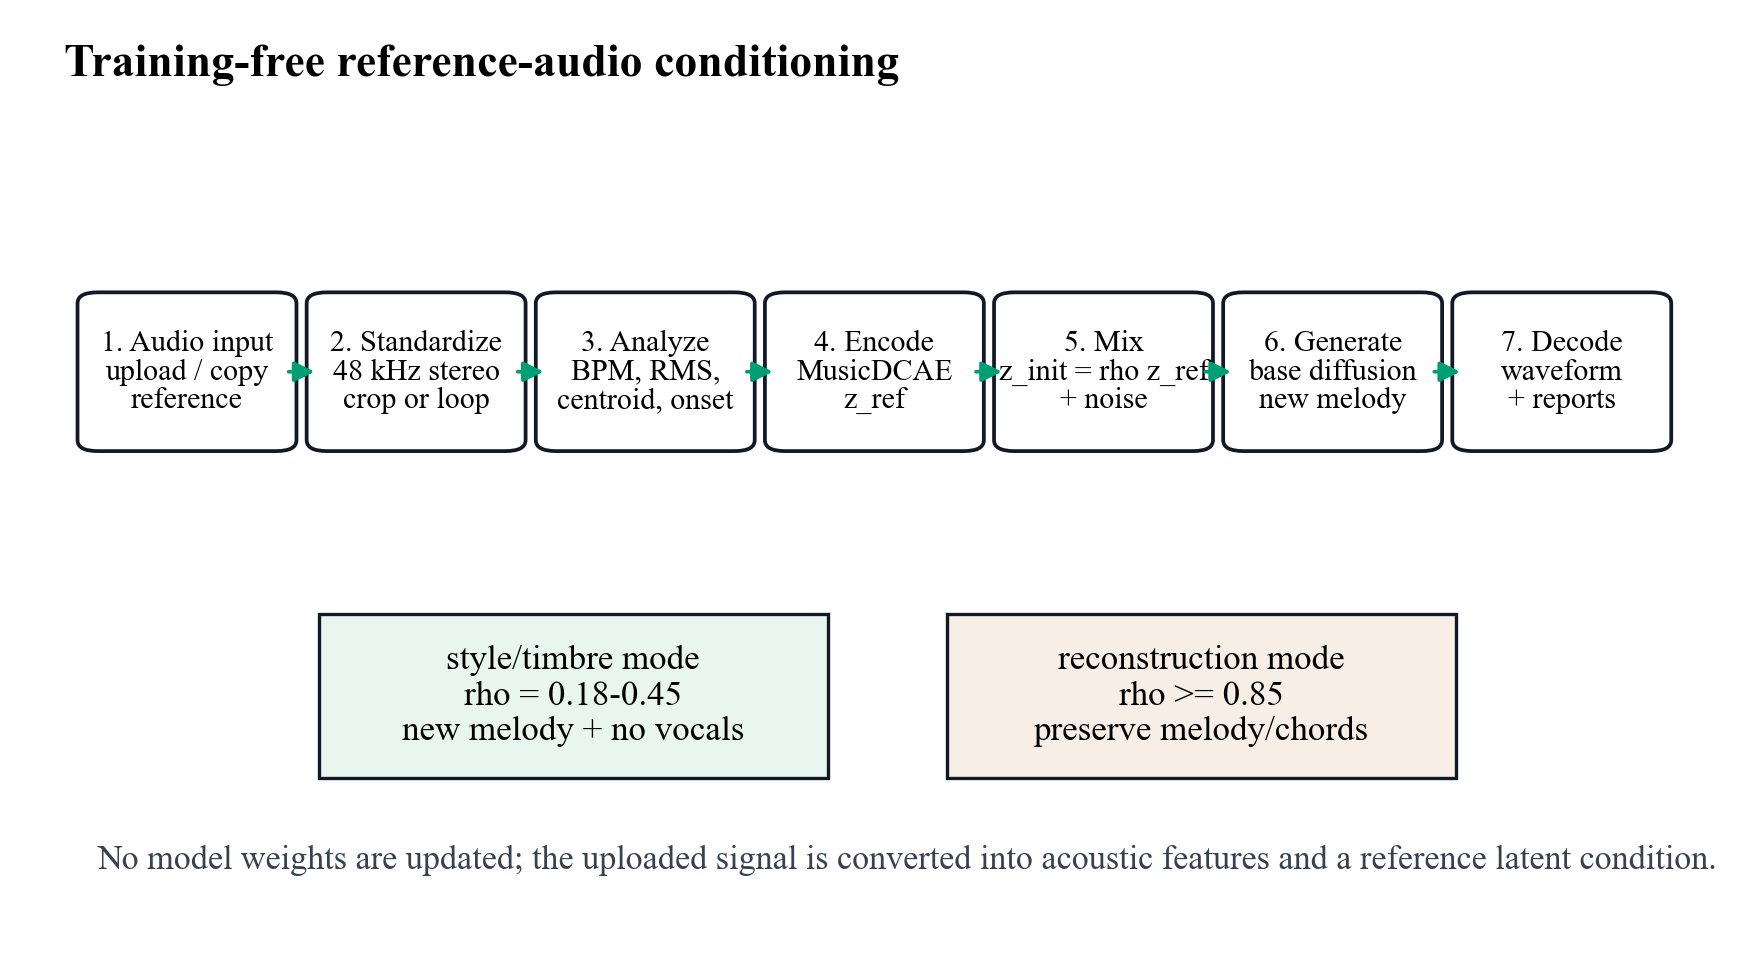
\includegraphics[width=0.92\linewidth]{assets/fig3_reference_conditioning.png}
\caption{无训练参考音频条件生成流程。参考音频进入模型前先被转换为声学特征和参考 latent，而不是只提取文本提示词。}
\end{figure}
\begin{equation}
z_{\mathrm{init}}=\rho z_{\mathrm{ref}}+\sqrt{1-\rho^2}\epsilon,\quad 0\leq\rho\leq 1
\end{equation}
式(4)表示参考 latent 与随机噪声的混合。ρ 越大，输出越接近参考音频，旋律和和弦复制风险越高；ρ 越小，新旋律自由度越高，但音色相似性下降。最近一次参考任务记录的参考 BPM 为 120.19，低频比例为 0.700，参考片段时长为 25.0 s。

为避免用户把无训练参考音频误解为“复制一首歌再改一点”，系统将参考模式分成两类。第一类是 style\_timbre，新旋律模式，只允许低强度参考 latent 影响音色、鼓组和混音质感；第二类是 reconstruction，重构模式，用于检查编码和解码链路是否能保留原始结构。论文实验默认使用第一类模式，并在网页上把 ref\_strength 的可用范围限制为较低区间。

\begin{table}[H]
\centering
\caption{参考音频条件生成模式}
\small
\begin{tabular}{p{0.22\linewidth}p{0.32\linewidth}p{0.36\linewidth}}
\toprule
模式 & ref\_strength & 技术含义 \\
\midrule
风格音色（新旋律） & 0.18-0.45 & 参考 latent 只提供音色和频谱约束，旋律由随机噪声与文本条件重新生成 \\
参考重构 & >=0.85 & 用于重建或诊断，可能保留原旋律和和弦，不作为新作品生成默认值 \\
纯文本基线 & 0 & 关闭参考音频，只使用 ACE-Step baseline 或 LoRA 文本生成 \\
去旋律代理 & 默认开启 & 用 HPSS/Demucs 降低主旋律和人声进入参考 latent 的强度 \\
多候选筛选 & 默认 2 个候选 & 按清晰度、低频比例、onset 和噪声惩罚自动选择输出 \\
\bottomrule
\end{tabular}
\end{table}
\begin{table}[H]
\centering
\caption{无训练参考音频条件生成流程}
\small
\begin{tabular}{p{0.22\linewidth}p{0.32\linewidth}p{0.36\linewidth}}
\toprule
步骤 & 处理内容 & 目的 \\
\midrule
1 & 读取上传音频并统一采样率、声道和时长 & 降低输入格式差异 \\
2 & 提取 BPM、RMS、低频比例、谱质心和 onset 密度 & 获得可解释声学条件 \\
3 & 构造去旋律参考代理音频 & 保留鼓、低频和质感，削弱旋律/人声复制 \\
4 & 通过 MusicDCAE 编码参考 latent & 保留细粒度音色和混音纹理 \\
5 & 按式(4)混合 z\_ref 与随机噪声 & 控制相似性与新旋律自由度 \\
6 & 生成多个候选并按客观清晰度评分 & 降低单 seed 失败和低频浑浊概率 \\
7 & 保存 wav、参数 JSON、波形图、频谱图和 latent trace & 支持复现实验与错误分析 \\
\bottomrule
\end{tabular}
\end{table}
\begin{figure}[H]
\centering
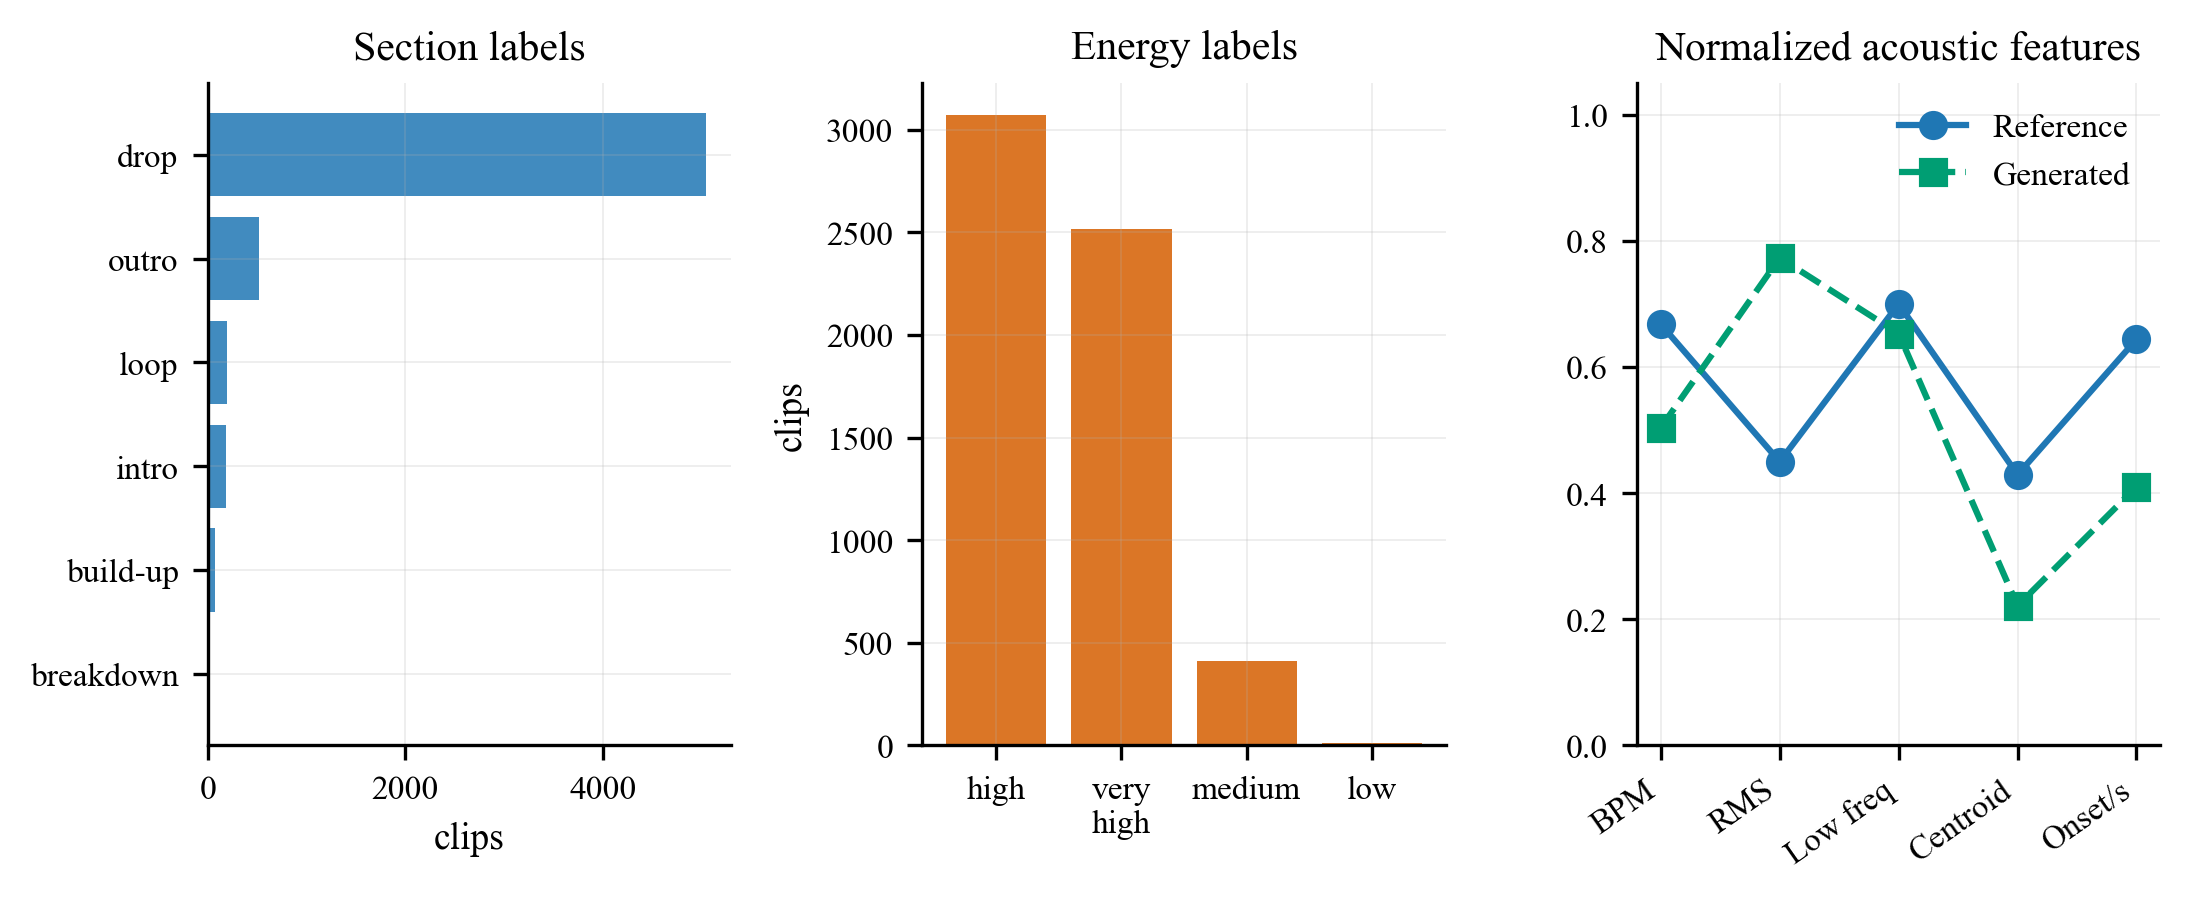
\includegraphics[width=0.92\linewidth]{assets/fig4_reference_features.png}
\caption{数据标签分布与参考音频声学特征。该图用于观察训练数据结构以及参考条件是否主要作用于非旋律声学属性。}
\end{figure}
\subsection{过程可视化与任务队列}
网页端将每次生成保存为独立任务目录，包括 task.json、status.txt、日志、wav、输入参数 JSON、参考音频副本、波形图、频谱图、响度包络、denoising trace 和 latent contact sheet。任务队列默认并发数设置为 2，因此当用户勾选基线对比时，LoRA 任务与 baseline 任务会作为两个独立任务同时进入线程池执行。这样可以回答三个实验问题：本次任务是否加载 LoRA，采样步数是否按设置执行，输出音频是否出现能量塌缩、削波或频谱混浊。

过程可视化的设计目标不是做装饰性界面，而是把扩散采样中原本不可见的中间状态转化为可检查证据。例如，denoising trace 可以显示每个保存步的 latent 均值、分位数和变化趋势；latent contact sheet 可以观察低维投影是否逐步形成稳定纹理；波形和频谱图可以揭示听感问题对应的信号形态。当用户认为生成“很糊”时，系统不只给出最终 wav，还能提供低频比例、谱图能量堆积和去噪轨迹作为定位依据。

\begin{table}[H]
\centering
\caption{网页生成过程可视化组件}
\small
\begin{tabular}{p{0.22\linewidth}p{0.32\linewidth}p{0.36\linewidth}}
\toprule
组件 & 记录内容 & 诊断价值 \\
\midrule
任务队列 & pending/running/done/error 状态，并发数=2 & LoRA 与 baseline 对比任务可同时生成，避免串行等待 \\
参数 JSON & seed、infer\_step、guidance、LoRA、reference & 复现实验条件，定位设置错误 \\
denoising trace & latent 均值、分位数、步数 & 检查采样是否真实执行足够步数 \\
latent contact sheet & 若干采样阶段的 latent 快照 & 观察生成结构是否逐步稳定 \\
波形/频谱图 & 幅度、频率、低频堆积 & 诊断音质、削波、浑浊和能量异常 \\
\bottomrule
\end{tabular}
\end{table}
\begin{equation}
m_s=\frac{1}{N}\sum_{i=1}^{N}|z_{s,i}|,\quad p95_s=P_{95}(|z_s|)
\end{equation}
\begin{figure}[H]
\centering
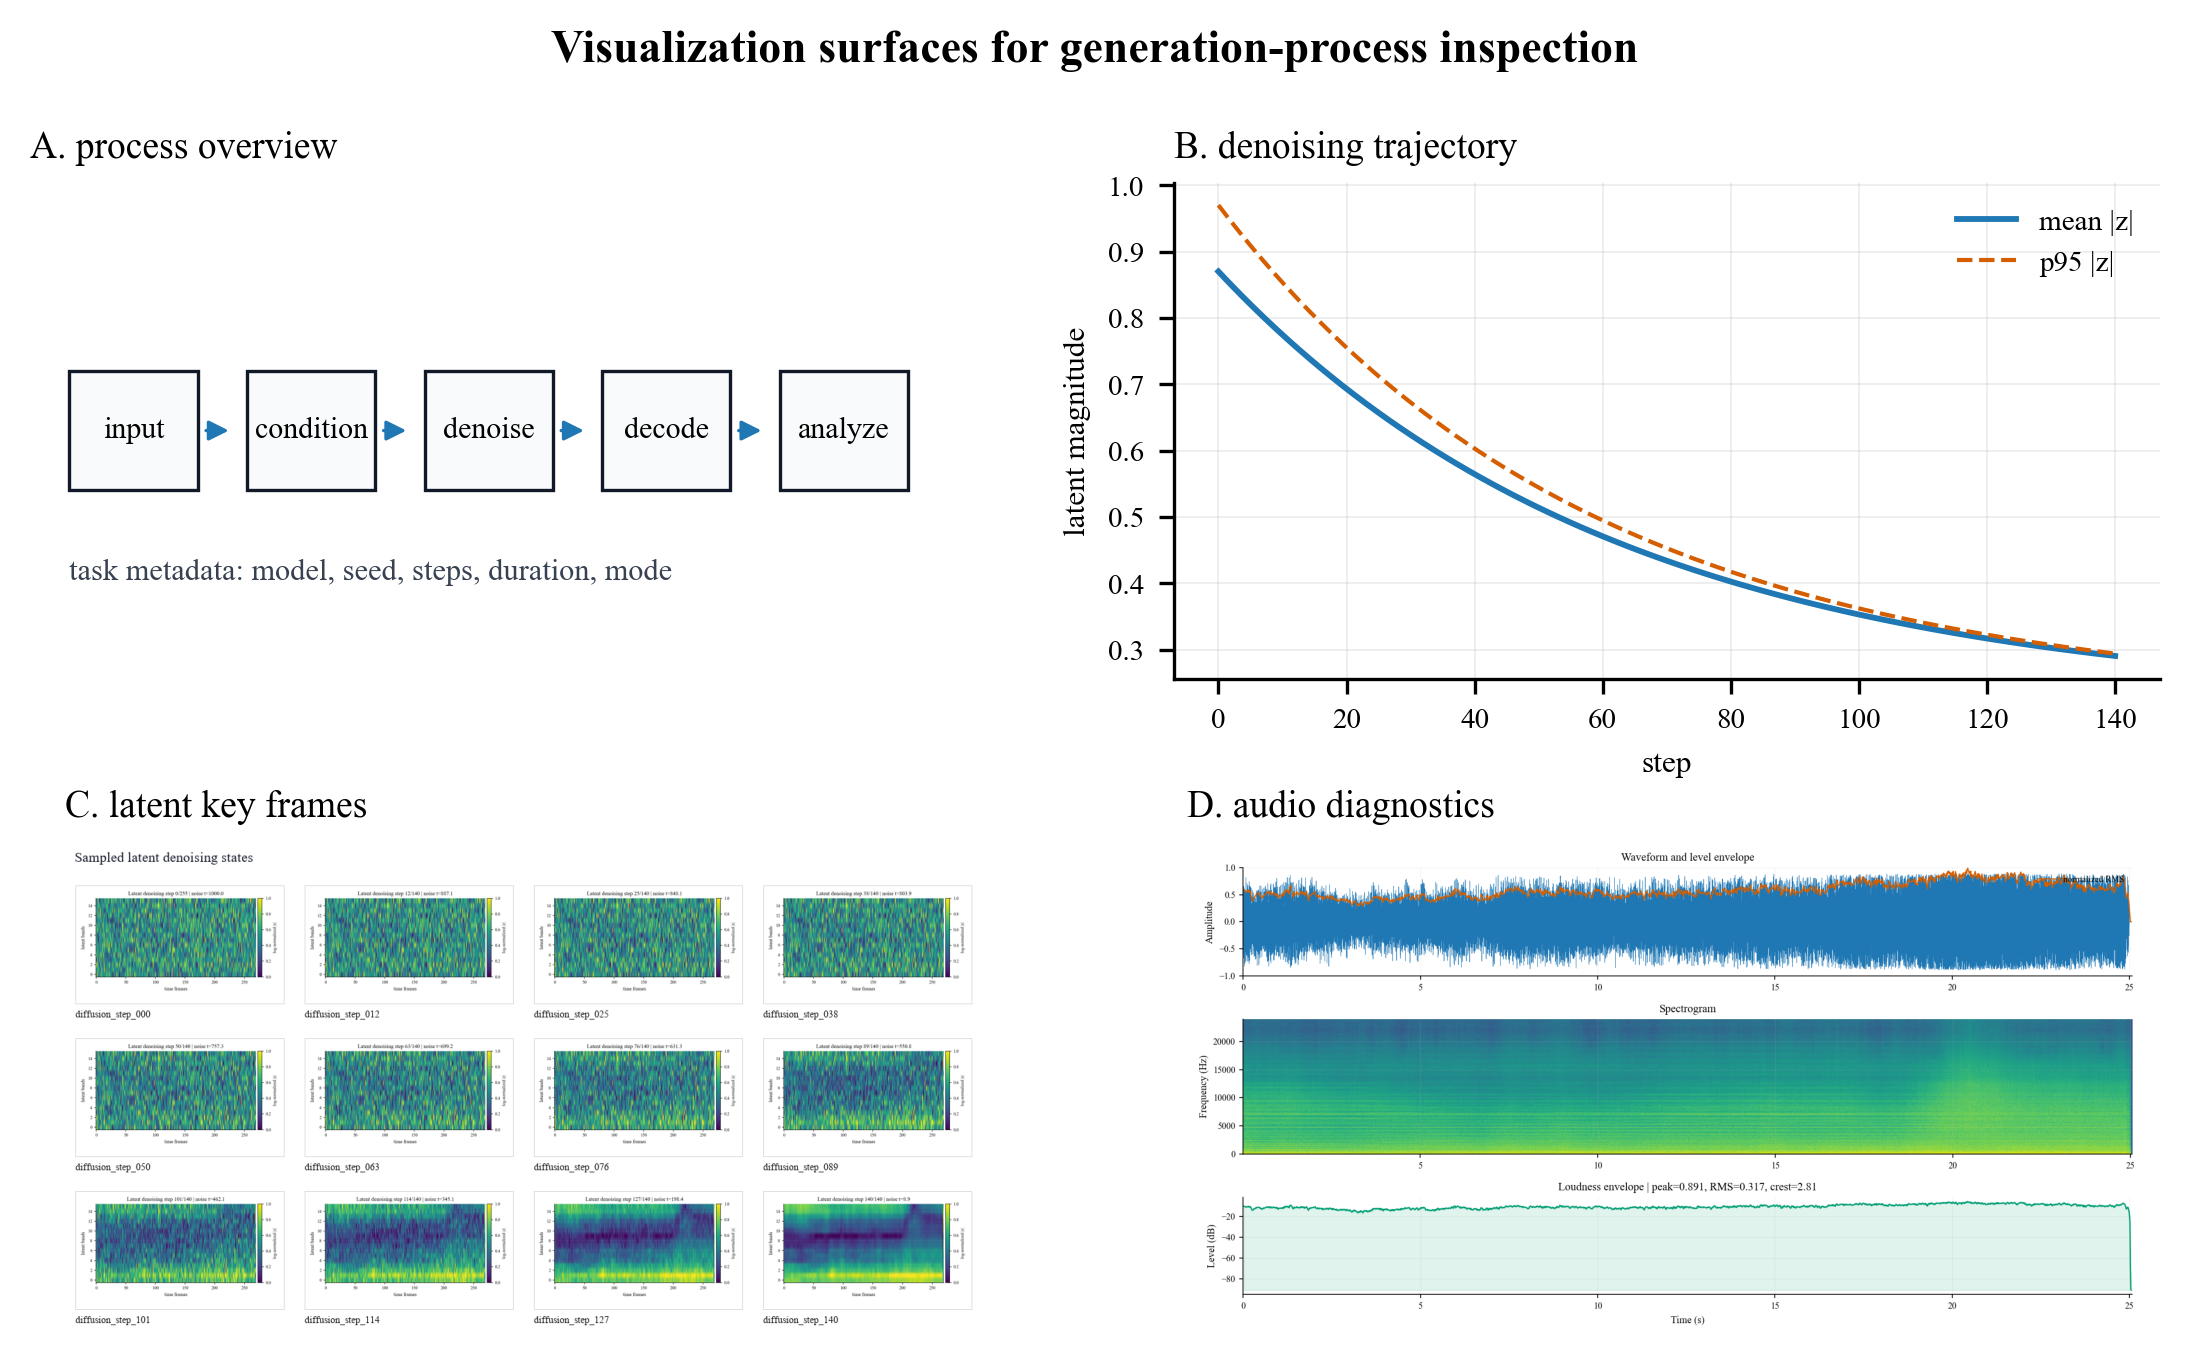
\includegraphics[width=0.92\linewidth]{assets/fig5_latent_visualization.png}
\caption{网页任务队列保存的生成过程可视化。包括流程概览、去噪轨迹、latent 关键帧和音频诊断图。}
\end{figure}
\section{实验}
\subsection{实验设置}
\begin{table}[H]
\centering
\caption{实验设置}
\small
\begin{tabular}{p{0.22\linewidth}p{0.32\linewidth}p{0.36\linewidth}}
\toprule
项目 & 设置 & 说明 \\
\midrule
基础模型 & ACE-Step v1-3.5B & MusicDCAE + UMT5 + 扩散 Transformer \\
数据集 & 6016 clips & train/val/test=4833/557/626 \\
训练硬件 & 4 x RTX 4090 & 本地工作站，总显存 96GB \\
LoRA 配置 & r=8, alpha=16 & dropout=0.01 \\
续训设置 & 120->960 & lr=2e-4, warmup=40, clip=0.35 \\
推理设置 & duration=15 s & infer\_step=120, guidance=12, weight=1.15 \\
对比方法 & ACE-Step baseline & 同 seed、同 prompt、同采样器 \\
指标 & RMS/低频/BPM/onset & 结合 waveform、spectrogram 与 latent trace \\
\bottomrule
\end{tabular}
\end{table}
实验设置遵循两个原则。首先，baseline 与 LoRA 对比必须固定随机种子和采样参数，否则不同初始噪声会掩盖 adapter 的真实影响。其次，参考音频模式不与 LoRA 微调同时启用，因为二者分别改变推理初态和模型参数，混合后很难解释输出差异。所有生成任务完成后，系统自动保存音频文件与指标 JSON，并生成同目录下的诊断图。

\subsection{评估指标与统计记录}
本文没有把单个指标作为最终音质结论，而是构建一组互补的诊断量。RMS 用于描述整体能量，低频比例用于描述 kick 与 bass 的能量占比，BPM 用于检查节奏条件是否被执行，onset 密度用于估计节奏事件数量，谱图用于观察频率分布是否出现低频堆积或高频缺失。对于扩散采样，latent trace 记录每个阶段的均值和 95 分位数，用于确认去噪过程是否逐步稳定。

\begin{equation}
\mathrm{RMS}=\sqrt{\frac{1}{T}\sum_{t=1}^{T}x_t^2},\quad R_{low}=\frac{\sum_{f<250Hz}|X(f)|^2}{\sum_f |X(f)|^2}
\end{equation}
\begin{table}[H]
\centering
\caption{客观指标与听感问题的对应关系}
\small
\begin{tabular}{p{0.22\linewidth}p{0.32\linewidth}p{0.36\linewidth}}
\toprule
指标或图像 & 异常表现 & 可能原因 \\
\midrule
RMS & 过低或波动过大 & 响度不足、生成能量不稳定或后处理过强 \\
低频比例 & 明显高于同类样本 & kick/bass 堆积，听感低频发糊 \\
BPM & 偏离 prompt 目标 & 节奏条件未被充分执行或 onset 检测失败 \\
onset 密度 & 过低或过高 & 节奏过稀、噪声瞬态过多或鼓组不清晰 \\
spectrogram & 中高频纹理缺失 & 音色不清晰、采样不足或参考强度过高 \\
latent trace & 均值长期不收敛 & 去噪步数不足、scheduler 设置不合适或 seed 初态较差 \\
\bottomrule
\end{tabular}
\end{table}
\subsection{主实验结果}
训练完成后，系统自动对 seed=7 和 seed=42 进行同 seed 对比。每个 seed 生成一首 baseline 和一首 LoRA 音频，prompt、duration、infer\_step、guidance\_scale、omega\_scale 和 scheduler 均保持一致。这种设计避免把随机初始噪声造成的差异误判为 LoRA 效果。

\begin{figure}[H]
\centering
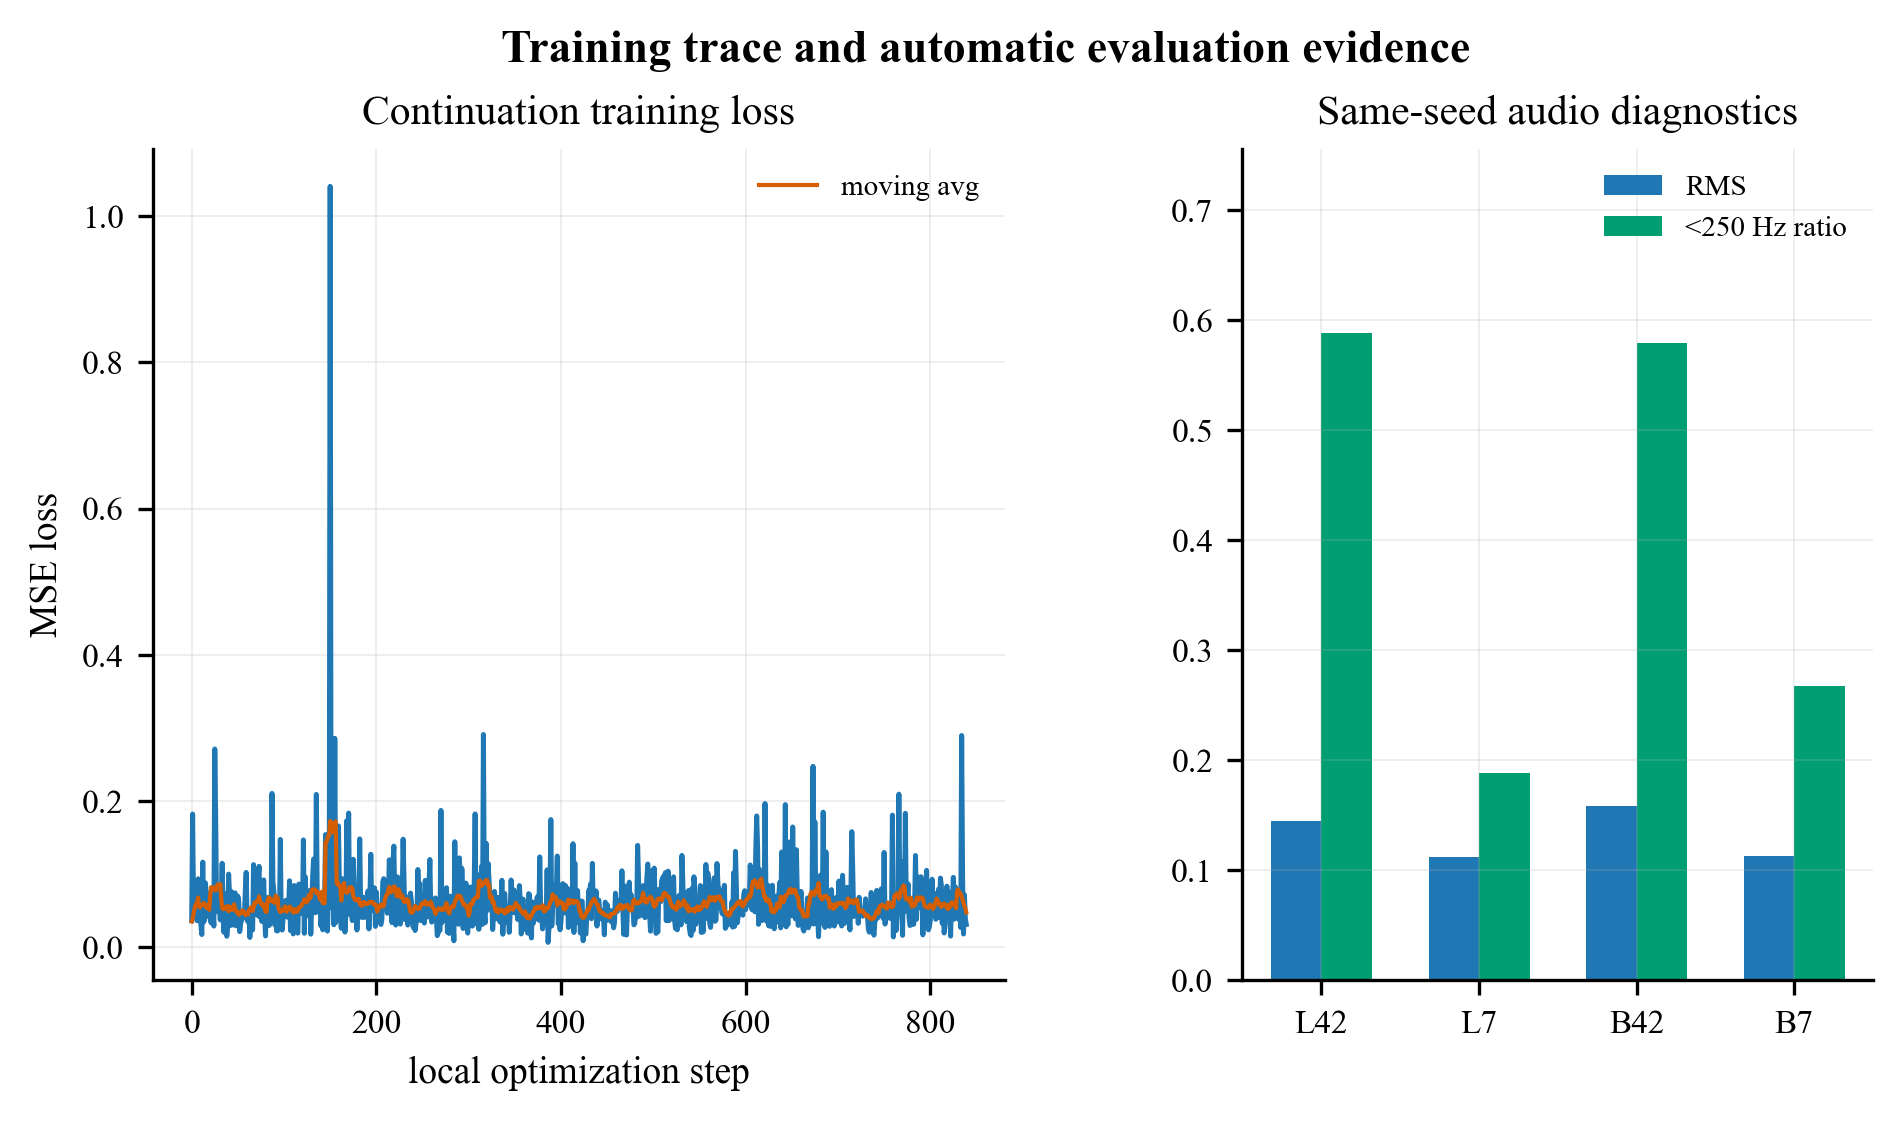
\includegraphics[width=0.92\linewidth]{assets/fig6_training_and_eval.png}
\caption{续训损失曲线与自动评估音频诊断。左图为 step=120 到 step=960 的训练损失，右图为同 seed baseline/LoRA 的 RMS 与低频比例。}
\end{figure}
\begin{table}[H]
\centering
\caption{同 seed 评估音频的客观指标}
\small
\begin{tabular}{p{0.22\linewidth}p{0.32\linewidth}p{0.36\linewidth}}
\toprule
样本 & RMS / 低频比例 & BPM / onset/s \\
\midrule
LoRA seed42 & 0.1447 / 0.5882 & 127.8 / 7.624 \\
LoRA seed7 & 0.1117 / 0.1884 & 127.8 / 4.213 \\
Base seed42 & 0.1583 / 0.5793 & 127.8 / 7.289 \\
Base seed7 & 0.1131 / 0.2673 & 127.8 / 5.149 \\
\bottomrule
\end{tabular}
\end{table}
表5 修正了早期版本中文件名过长导致的表格重叠问题，使用短标签表示音频样本。结果显示四个样本的估计 BPM 均为 127.8，说明 prompt 中 128 BPM 的节奏条件基本被执行；不同 seed 的低频比例和 onset 密度差异较大，反映扩散初始噪声会影响节奏骨架和频谱分离。因此，本文后续分析不把 seed 大小解释为音质单调规律，而把 seed 视为随机初态变量。

从自动指标看，LoRA 与 baseline 的差异并不一定表现为 BPM 的变化，因为 BPM 强约束主要来自 prompt 和采样条件；更有意义的是低频比例、onset 密度和谱图纹理的变化。若 LoRA 输出在相同 seed 下表现出更明确的低频结构或更接近目标数据的瞬态密度，说明 adapter 已经影响扩散去噪中的局部声学决策。若听感上仍然浑浊，则需要结合表8检查是否为采样步数不足、LoRA 权重过高或后处理链过强。

\subsection{消融实验与参数分析}
\begin{table}[H]
\centering
\caption{消融实验设计}
\small
\begin{tabular}{p{0.22\linewidth}p{0.32\linewidth}p{0.36\linewidth}}
\toprule
实验 & 变量 & 预期观察 \\
\midrule
A0 Baseline & 不加载 LoRA & 作为通用 ACE-Step 生成参考 \\
A1 Early LoRA & step=120, last 2 blocks & 验证早期轻量 adapter 是否产生风格偏移 \\
A2 Continued LoRA & step=960, last 4 blocks & 验证更深末端层和更长训练是否改善稳定性 \\
A3 Reference-low & ρ=0.18-0.45 & 音色迁移但降低旋律复制 \\
A4 Reference-high & ρ>=0.85 & 接近重构，检查旋律/和弦复制倾向 \\
A5 No-lyrics & lyrics=[instrumental] & 检查无歌词时是否减少人声泄漏 \\
\bottomrule
\end{tabular}
\end{table}
\begin{table}[H]
\centering
\caption{关键参数影响分析}
\small
\begin{tabular}{p{0.22\linewidth}p{0.32\linewidth}p{0.36\linewidth}}
\toprule
参数 & 增大时的影响 & 本文设置 \\
\midrule
LoRA weight & 风格偏移增强，但过高可能破坏基础音质 & 1.15 \\
infer\_step & 去噪更充分，推理时间增加 & 120；参考模式默认 140 \\
guidance\_scale & 文本约束更强，过高会压缩自然度 & 10-12 \\
ref\_strength & 音色相似性增强，但旋律复制风险上升 & 0.35，限制 0.18-0.45 \\
seed & 改变初始 latent 和早期节奏骨架 & 固定 seed 做对照 \\
\bottomrule
\end{tabular}
\end{table}
消融实验的重点是确认每个模块的作用边界。A1 与 A2 比较训练深度和续训步数的影响；A3 与 A4 比较参考强度对音色迁移和旋律复制的影响；A5 单独检查歌词为空时的人声泄漏问题。本文没有把所有消融都写成最终数值排行榜，因为音乐生成结果高度依赖听感和随机初态，更合理的做法是保存同 seed 音频、客观指标和诊断图，让每个结论都能回到可播放样本。

\subsection{可视化示例与错误分析}
可视化结果用于定位生成失败原因。当 denoising trace 的 mean |z| 长时间不下降时，通常意味着去噪过程未充分收敛；当谱图低频区域过亮且中高频纹理模糊时，听感上容易表现为低频糊成一团；当 waveform 峰值接近 1 且 RMS 异常低时，可能存在瞬态尖峰而非稳定响度。这些证据不能完全替代人工听评，但能帮助区分模型条件失效、采样步数不足、后处理过强和随机 seed 不佳等不同问题。

失败案例主要分为三类。第一类是音质浑浊，常见于低频比例过高或参考强度过高；第二类是旋律不清晰，可能来自采样步数不足、guidance 过强或 seed 初态较差；第三类是风格不够还原，通常说明 LoRA 训练步数或数据覆盖仍不足。对于第一类问题，优先降低 ref\_strength 或减弱低频后处理；对于第二类问题，优先提高 infer\_step 并检查 latent trace；对于第三类问题，则需要继续训练或扩展目标数据集。

\section{讨论}
\subsection{LoRA 微调与参考条件的分工}
在本地 4 卡 RTX 4090 工作站上，本文方法的优势是训练参数量小、权重产物轻量，且不会破坏 ACE-Step 原始能力。LoRA 续训适合固定风格长期复用；无训练参考音频适合临时上传样本并迁移音色和混音质感。二者必须分离，因为一个改变模型参数，另一个改变推理初态；混用会导致无法判断差异来自 adapter、参考 latent 还是随机 seed。

从建模角度看，LoRA 学到的是目标数据域在扩散去噪网络中的参数化偏移，适合表达稳定、可复用的风格先验；参考音频条件表达的是单个上传样本的局部声学状态，适合迁移一次性的音色和混音质感。如果用户追求“长期固定风格”，应优先使用 LoRA；如果用户只是临时给出一段参考曲，希望得到相似音色但不同旋律，则应使用参考音频路径。

\subsection{与直接提示词方法的差异}
直接提示词方法的优点是简单，但它无法读取参考音频中的真实声学结构。例如，同样写作“bright piano, sidechain bass, progressive house drop”，不同参考曲的低频能量、瞬态密度、混响空间和高频纹理仍可能完全不同。本文的无训练路径至少保留了两类信号证据：低维特征用于描述可解释属性，高维 latent 用于携带难以文本化的音色纹理。因此，它比纯 prompt 更接近智能语音处理中的信号驱动生成。

但是，参考 latent 不是旋律/和声的完美解耦表示。过高的 ref\_strength 会把旋律轮廓、和弦运动和局部节奏一起带入生成，使输出听起来像原曲重构；过低的 ref\_strength 又会削弱音色相似性。本文采用低强度参考加特征补偿的策略，本质上是在相似性与新颖性之间折中。后续若要进一步提高控制精度，需要引入旋律轮廓分离、和弦估计或 stem 级参考编码。

\subsection{训练架构改变带来的影响}
本次架构改变主要体现在三点：可训练 block 数由 2 扩展到 4，继续训练时从 step=120 adapter 初始化，训练超参数改为更保守的低学习率和更长 warmup。这些改变共同指向一个目标：让 adapter 在更长的去噪链路中形成稳定风格偏移，而不是只在最终输出层附近做强行补偿。从工程角度看，参数量由约 1.12M 增加到约 2.02M，仍然只占基础模型极小比例，权重文件和加载成本依旧可控。

需要注意的是，增加可训练层数并不必然提高音质。如果学习率过高或训练数据覆盖不足，更大的 adapter 也可能学习到噪声、局部片段或数据偏差。因此本文没有把可训练范围无限扩大，而是只扩展到末端 4 个 block，并保持 MusicDCAE、UMT5 和主体大部分 Transformer 冻结。这种方案在风格表达能力、训练稳定性和实验成本之间较为平衡。

\subsection{局限性与后续研究方向}
局限也很明确。第一，step=960 仍属于有限轮数续训，不能保证完整学习目标艺术家的全部风格结构；第二，ACE-Step 的 audio2audio 更接近参考 latent 重采样，并非专门的旋律/和声解耦模型，因此“音色一致但旋律完全不同”只能近似实现；第三，本文的评价仍以客观诊断和少量同 seed 听感对照为主，尚未完成大规模人工主观实验和统计显著性检验。未来可加入旋律轮廓分离、和弦估计、鼓组/低频 stem 特征提取、reference adapter 训练和基于 CLAP/MERT 的感知相似度评分。

在实验评价上，后续还可以引入三类更严格的评估。第一是主观听评，让多名听众分别评价音质、旋律清晰度、风格相似性和新颖性；第二是分布级客观指标，如 FAD 或基于预训练音频分类器的嵌入距离；第三是可解释结构指标，如鼓点稳定性、和弦变化率、低频侧链周期和段落边界准确性。这些指标可以与本文已有的同 seed 任务队列结合，形成更完整的智能音频生成评价体系。

在系统实现上，后续可把训练、推理和评估拆成更明确的流水线：训练端负责生成 adapter 和 manifest；推理端只读取已发布 adapter；评估端统一生成指标和图表。这样可以避免网页推理逻辑和训练逻辑互相污染，也方便未来把 GPU 训练迁移到服务器或多机环境。对于课程项目而言，当前实现已经覆盖从音频预处理到模型适配、生成、后处理和可视化报告的完整闭环。

\section{结论}
本文面向智能语音处理课程，构建了一个基于 ACE-Step 的音乐风格生成系统。核心发现包括：1）在冻结基础模型的前提下，4-block LoRA 续训可以把可训练参数控制在约 2.02M 并实现真实风格适配；2）上传参考音频可以通过标准化、特征提取和 MusicDCAE latent 条件进入生成过程，而不是退化为提示词工程；3）同 seed 对照、latent trace、波形和频谱可视化能显著提升生成实验的可复现性和可解释性。后续工作将重点扩展 GPU 训练轮数、引入专用 reference adapter、建立人工听评和客观感知指标联合评价。

\section*{参考资料}
\begin{enumerate}[leftmargin=2em]
\item Ho J, Jain A, Abbeel P. Denoising Diffusion Probabilistic Models[C]//Advances in Neural Information Processing Systems. 2020.
\item Rombach R, Blattmann A, Lorenz D, Esser P, Ommer B. High-Resolution Image Synthesis with Latent Diffusion Models[C]//Proceedings of the IEEE/CVF Conference on Computer Vision and Pattern Recognition. 2022.
\item Liu H, Chen Z, Yuan Y, et al. AudioLDM: Text-to-Audio Generation with Latent Diffusion Models[C]//International Conference on Machine Learning. 2023.
\item Liu H, Tian Q, Yuan Y, et al. AudioLDM 2: Learning Holistic Audio Generation with Self-supervised Pretraining[C]//International Conference on Learning Representations. 2024.
\item Copet J, Kreuk F, Gat I, et al. Simple and Controllable Music Generation[C]//Advances in Neural Information Processing Systems. 2023.
\item Agostinelli A, Denk T I, Borsos Z, et al. MusicLM: Generating Music From Text[J/OL]. arXiv:2301.11325, 2023.
\item Gong J, Zhao W, Wang S, Xu S, Guo J. ACE-Step: A Step Towards Music Generation Foundation Model[J/OL]. arXiv:2506.00045, 2025.
\item Hu E J, Shen Y, Wallis P, et al. LoRA: Low-Rank Adaptation of Large Language Models[C]//International Conference on Learning Representations. 2022.
\item Défossez A, Copet J, Synnaeve G, Adi Y. High Fidelity Neural Audio Compression[J]. Transactions on Machine Learning Research, 2023.
\item Elizalde B, Deshmukh S, Al Ismail M, Wang H. CLAP: Learning Audio Concepts from Natural Language Supervision[C]//IEEE International Conference on Acoustics, Speech and Signal Processing. 2023.
\item Li Y, Yuan R, Zhang G, et al. MERT: Acoustic Music Understanding Model with Large-Scale Self-supervised Training[J/OL]. arXiv:2306.00107, 2023.
\item McFee B, Raffel C, Liang D, et al. librosa: Audio and Music Signal Analysis in Python[C]//Proceedings of the 14th Python in Science Conference. 2015.
\item Kilgour K, Zuluaga M, Roblek D, Sharifi M. Fréchet Audio Distance: A Reference-Free Metric for Evaluating Music Enhancement Algorithms[C]//Interspeech. 2019.
\item Kong Q, Cao Y, Iqbal T, Wang Y, Wang W, Plumbley M D. PANNs: Large-Scale Pretrained Audio Neural Networks for Audio Pattern Recognition[J]. IEEE/ACM Transactions on Audio, Speech, and Language Processing, 2020, 28: 2880-2894.
\end{enumerate}
\end{document}